% --------------------------------------
% Document Class
% --------------------------------------
\documentclass[a4paper,11pt]{article}
% --------------------------------------



% --------------------------------------
% Use Package
% --------------------------------------


%\usepackage[francais]{babel}
%\usepackage{ucs}
\usepackage[utf8]{inputenc}
\usepackage[T1]{fontenc}

\usepackage{makeidx}
\usepackage{color}
\usepackage{graphicx}
\usepackage{float}
\usepackage[hidelinks]{hyperref} 
\usepackage{geometry}
%\usepackage{lastpage}
%\usepackage{marginnote}
\usepackage{fancyhdr}
%\usepackage{titlesec}
%\usepackage{framed}
\usepackage{amsmath}
\usepackage{empheq}
\usepackage{array}
\usepackage{multicol}
\usepackage{csquotes}
%\usepackage{adjustbox}

% insert code
\usepackage{listings}

% define our color
\usepackage{xcolor}

% code color
\definecolor{ligthyellow}{RGB}{250,247,220}
\definecolor{darkblue}{RGB}{5,10,85}
\definecolor{ligthblue}{RGB}{1,147,128}
\definecolor{darkgreen}{RGB}{8,120,51}
\definecolor{darkred}{RGB}{160,0,0}

% other color
\definecolor{ivi}{RGB}{141,107,185}

\def\verticaltext#1{\rotatebox[origin=c]{90}{\x{#1}}}


\lstset{
    language=C++,
    captionpos=b,
    extendedchars=true,
    frame=lines,
    numbers=left,
    numberstyle=\tiny,
    numbersep=5pt,
    keepspaces=true,
    breaklines=true,
    showspaces=false,
    showstringspaces=false,
    breakatwhitespace=false,
    stepnumber=1,
    showtabs=false,
    tabsize=3,
    basicstyle=\small\ttfamily,
    backgroundcolor=\color{ligthyellow},
    keywordstyle=\color{ligthblue},
    morekeywords={include, printf, uchar},
    identifierstyle=\color{darkblue},
    commentstyle=\color{darkgreen},
    stringstyle=\color{darkred},
}


% --------------------------------------



% --------------------------------------
% Page setting
% --------------------------------------
%\pagestyle{empty}
\setlength{\headheight}{15pt}

\setcounter{secnumdepth}{3}
\setcounter{tocdepth}{2}

\makeatletter
\@addtoreset{chapter}{part}
\makeatother 

\hypersetup{         % parametrage des hyperliens
  colorlinks=true,      % colorise les liens
  breaklinks=true,      % permet les retours à la ligne pour les liens trop longs
  urlcolor= blue,       % couleur des hyperliens
  linkcolor= black,     % couleur des liens internes aux documents (index, figures, tableaux, equations,...)
  citecolor= green      % couleur des liens vers les references bibliographiques
}

% --------------------------------------

% --------------------------------------
% Information
% --------------------------------------
\title{
  \noindent\hrulefill \\
  \vspace{10mm} Compte-rendu TP3 VisA: Rectification épipolaire et stéréovision dense
}

\author{Gaëtan DEFLANDRE}
% --------------------------------------

\definecolor{myColor}{rgb}{0.5, 0.1, 0.75}

% --------------------------------------
% Begin content
% --------------------------------------
\begin{document}


\maketitle

\noindent\hrulefill \\


\section{Introduction}
Dans le cadre du second TP, nous avons étudié la géométrie épipolaire. Ainsi, nous avons
effectué une mise en correspondance stéréoscopique. \\

Dans ce troisième TP, nous travaillons sur la stéréovision dense, qui consiste à calculer 
la disparité, entre l'image de gauche et de droite, associée à chaque pixel. Pour cela, les 
images sont acquises avec un stéréoscope canonique, car les droites épipolaires associées à 
deux points homologues sont confondues. Dans le cas d'un stéréoscope non canonique, il faut 
passer par une étape de rectification épipolaire avant de calculer la disparité.\\

\newpage

\section{Fonctionnement général}

Nous utilisons des images acquises avec un stéréoscope canonique. L'une des propriétés 
intéressantes et que les droites épipolaires associées à deux points homologues sont 
confondues. En effet, avec cette configuration, de simplesdécalages horizontaux suffisent 
pour retrouver les points homologues.\\

\begin{figure}[H]
  \centering
  \shortstack{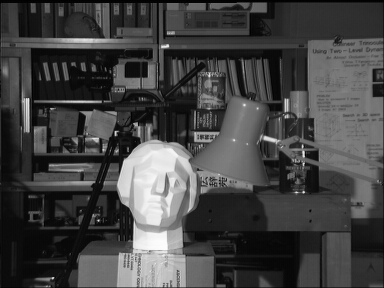
\includegraphics[width=200px]{../left.png} \\ Image de gauche}
  \shortstack{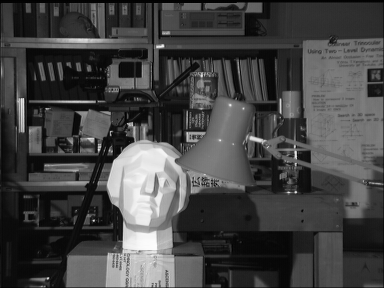
\includegraphics[width=200px]{../right.png} \\ Image de droite}
\end{figure}

La première double boucle de la fonction initialise la matrice
\textbf{mMinSSD} avec la valeur de $dMinSSD = (2 * iWindowHalfSize + 1)^2 * 512.0$. 
C'est-à-dire la dissimilarité maximum SSD: la somme des différences aux carrés (sum of squared 
differences).

\begin{lstlisting}[caption=Initialisation]
    // Initialisation de l'image du minimum de SSD
    dMinSSD = pow((double)(2 * iWindowHalfSize + 1), 2.0) * 512.0;
    for (iRow = iWindowHalfSize;
            iRow < mMinSSD.size().height - iWindowHalfSize;
            iRow++)
    {
        // Pointeur sur le debut de la ligne
        pdPtr1 = mMinSSD.ptr<double>(iRow);
        // Sauter la demi fenetre non utilisee
        pdPtr1 += iWindowHalfSize;
        // Remplir le reste de la ligne
        for (iCol = iWindowHalfSize;
                iCol < mMinSSD.size().width - iWindowHalfSize;
                iCol++)
            *pdPtr1++ = dMinSSD;
    }
\end{lstlisting}

\newpage

Les boucles qui suivent recherches pour chaque pixel de l'image de gauche le décalage qui 
minimise la disparité. Nous retrouvons le décalage minimum, par calcul de la dissimilarité
SSD (sum of squared differences).\\

Pour un point donné, la SSD minimum est calculé en parcourant les pixels avec la même 
abscisse que ce point. Pour chacun de ces points, une valeur SSD est calculée et stockée 
dans \textbf{mSDD}, une matrice tampon. Si cette valeur est minimale, nous la stockons 
dans \textbf{mMinSSD}.\\

Les valeurs des décalages sont stockées dans \textbf{mLeftDisparityMap}.\\


\begin{lstlisting}[caption=Retrouver dissimilarité minimum]
for (unsigned x=iWindowHalfSize; x<=cols; x++){
  for (unsigned y=iWindowHalfSize; y<=rows; y++){
    for (int i= -iWindowHalfSize; i<=iWindowHalfSize; i++){

      if (winX<0 || winX>=cols){
        // Si on est hors de l'image on passe
        continue;
      }
      for(int j=-iWindowHalfSize; j<=iWindowHalfSize; j++){

        winX = x + i;
        winY = y + j;

        if (winY<0 || winY>=rows){
          // Si on est hors de l'image on passe
          continue;
        }

        // Valeur image gauche
        double il = (double)mLeftGray.at<unsigned char>(winY,winX);
        // Valeur image droite
        double ir = (double)mRightGray.at<unsigned char>(winY,winX-iShift);

        ssd += pow(il-ir, 2.0);

      }
    }

    mLeftSSDCost.at<double>(y,x) = ssd;
    ssd = 0.0;
  }
}
\end{lstlisting}

\newpage


\section{Calculs des disparités gauches, puis droites}

La fonction \textbf{normalize} est utilisée pour que les images calculées 
utilisent tout l'histogramme des niveaux de gris. Après cela, nous distinguons 
les différents niveaux de gris car l'écart-type de l'histogramme plus élevé.

$$
normalize(mLeftDisparity, mLeftDisparity, 0, 255, CV\_MINMAX);
$$\\

Pour le calcul dissimilarité, nous utilisons la SDD (sum of squared differences) 
qui se sert qu'un voisinage dans l'image de gauche et droite.\\

Formule de la SSD:

$$
\sum_{i=-w_x}^{w_x} \sum_{i=-w_y}^{w_y} (I_l(x_l+i,y+j)-I_r(x_l+1-s,y+j))^2
$$

\begin{figure}[H]
  \centering
  \shortstack{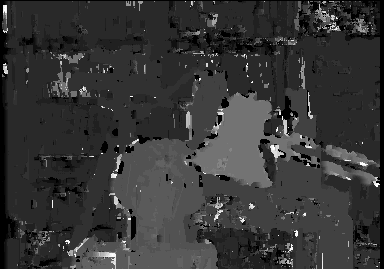
\includegraphics[height=140px]{../left_disparity.png} \\ Dissimilarité de gauche}
  \shortstack{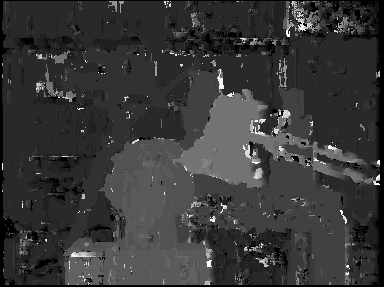
\includegraphics[height=140px]{../right_disparity.png} \\ Dissimilarité de droite}
\end{figure}

\newpage

\begin{lstlisting}[caption=Calcul de la SSD gauche]
    for (unsigned x=iWindowHalfSize; x<=cols; x++){
        for (unsigned y=iWindowHalfSize; y<=rows; y++){
            for (int i= -iWindowHalfSize; i<=iWindowHalfSize; i++){

                if (winX<0 || winX>=cols){
                    // Si on est hors de l'image on passe
                    continue;
                }

                for(int j=-iWindowHalfSize; j<=iWindowHalfSize; j++){

                    winX = x + i;
                    winY = y + j;

                    if (winY<0 || winY>=rows){
                        // Si on est hors de l'image on passe
                        continue;
                    }

                    // Valeur image gauche
                    double il = (double)mLeftGray.at<unsigned char>(winY,winX);
                    // Valeur image droite
                    double ir = (double)mRightGray.at<unsigned char>(winY,winX-iShift);

                    ssd += pow(il-ir, 2.0);

                }
            }

            mLeftSSDCost.at<double>(y,x) = ssd;
            ssd = 0.0;

        }
    }

    return mLeftSSDCost.clone();
\end{lstlisting}

\newpage

\begin{lstlisting}[caption=Calcul de la SSD droit]
    for (unsigned x=iWindowHalfSize; x<=cols; x++){
        for (unsigned y=iWindowHalfSize; y<=rows; y++){
            for (int i= -iWindowHalfSize; i<=iWindowHalfSize; i++){

                if (winX<0 || winX>=cols){
                    // Si on est hors de l'image on passe
                    continue;
                }

                for(int j=-iWindowHalfSize; j<=iWindowHalfSize; j++){

                    winX = x + i;
                    winY = y + j;

                    if (winY<0 || winY>=rows){
                        // Si on est hors de l'image on passe
                        continue;
                    }

                    // Valeur image gauche
                    double il = (double)mLeftGray.at<unsigned char>(winY,winX+iShift);
                    // Valeur image droite
                    double ir = (double)mRightGray.at<unsigned char>(winY,winX);

                    ssd += pow(ir-il, 2.0);

                }
            }

            mRightSSDCost.at<double>(y,x) = ssd;
            ssd = 0.0;

        }
    }

    return mRightSSDCost.clone();
\end{lstlisting}

\newpage

\section{Cohérence gauche-droite}

Il est possible de conserver uniquement les paires de pixels homologues qui sont 
identiques dans les deux images du stéréoscope. Cette technique nous permet d'enlever les 
faux appariements liés à l'occultation. Pour cela, nous recréons une carte de 
disparité à partir de la disparité de gauche et de droite. Cette nouvelle carte 
doit respecter les conditions suivantes:

$$
\begin{aligned}
d_r(x,y) &= d_l(x+d_r(x,y),y) \\
d_l(x,y) &= d_r(x-d_l(x,y),y) \\
\end{aligned}
$$


\begin{figure}[H]
  \centering
  \shortstack{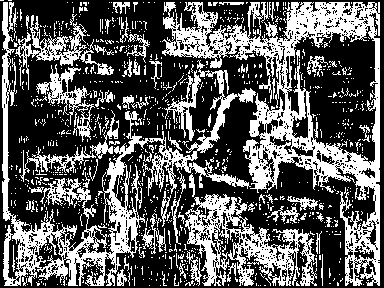
\includegraphics[width=200px]{../mask.png} \\ {\small Masque des disparités cohérente gauche-droite}}
  \shortstack{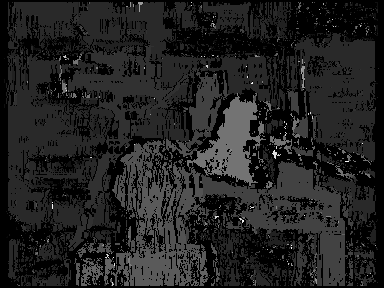
\includegraphics[width=200px]{../disparity.png} \\ {\small Disparité gauche-droite}}
\end{figure}

\begin{lstlisting}[caption=Fonction donnant la disparité cohérente gauche-droite]
/// \brief Verifie la coherence des cartes gauche et froite.
///
/// @param psLeftDisparity: carte gauche des disparites
/// @param psRightDisparity: carte droite des disparites
/// @param psDisparity: carte des disparites fusionnee
/// @param psValidityMask: carte des disparites valides
Mat iviLeftRightConsistency(const Mat& mLeftDisparity,
                            const Mat& mRightDisparity,
                            Mat& mValidityMask)
{
    Mat mDisparity(mLeftDisparity.size(), CV_8U);

    unsigned rows = mLeftDisparity.rows;
    unsigned cols = mLeftDisparity.cols;

    for (unsigned x=0; x<cols; x++) {
        for (unsigned y=0; y<rows; y++) {

            unsigned char dr1 = mRightDisparity.at<unsigned char>(y,x);
            unsigned char dl1 = mLeftDisparity.at<unsigned char>(y,x+dr1);

            unsigned char dl2 = mLeftDisparity.at<unsigned char>(y,x);
            unsigned char dr2 = mRightDisparity.at<unsigned char>(y,x-dl2);

            if(dr1==dl1 && dl2==dr2){
                mValidityMask.at<unsigned char>(y,x) = 0;
                mDisparity.at<unsigned char>(y,x) = dl2;
            } else {
                mValidityMask.at<unsigned char>(y,x) = 255;
                mDisparity.at<unsigned char>(y,x) = 0;
            }
        }
    }

    return mDisparity.clone();
}
\end{lstlisting}

\section{Conclusion}

Pour conclure, nous constatons qu'avec un stéréoscope canonique, nous pouvons effectuer 
une carte de disparité dense, cohérente pour l'image gauche et droite. Nous obtenons un 
résultat satisfaisant. Cependant, un nombre non négligeable de pixels restent sans disparité, 
lier aux phénomènes d'occultation et de bord.\\

En règle générale, la carte de disparité nous donne une notion de la profondeur de l'image. 
Avec une exception, pour les objets proches du stéréoscope, situé sur l'entraxe.\\


\end{document}
